\documentclass[uplatex,a4paper,10pt,dvipdfmx]{jsarticle}
\usepackage{preamble}
\usepackage{tikz}
\usepackage{gnuplot-lua-tikz} % gnuplot動作
\usepackage{info}

% \includegraphicsのためのpath (src/img下に画像を保存)
\graphicspath{{src/img}}

% \addbibresource{src/references.bib}

\title{Skelton File}
\author{\myid  \myname}
\date {2022年2月17日 作成\\\today{} 更新}

\begin{document}
\maketitle

\section{目的}
hogeとは,fooを表現する物理量である.
...

今回の実験の目的は,barを求めることである.

\section{実験の原理}
% Point: 用いた物理的原理を数式を交えて書く

\section{方法}
この実験では以下のような装置(図\ref{fig:experiment-blender-nbg} 参照)を用いて測定を行なった.
<実験装置名>は<目的>という目的で使い,....ができる.

\begin{figure}[H]\centering
  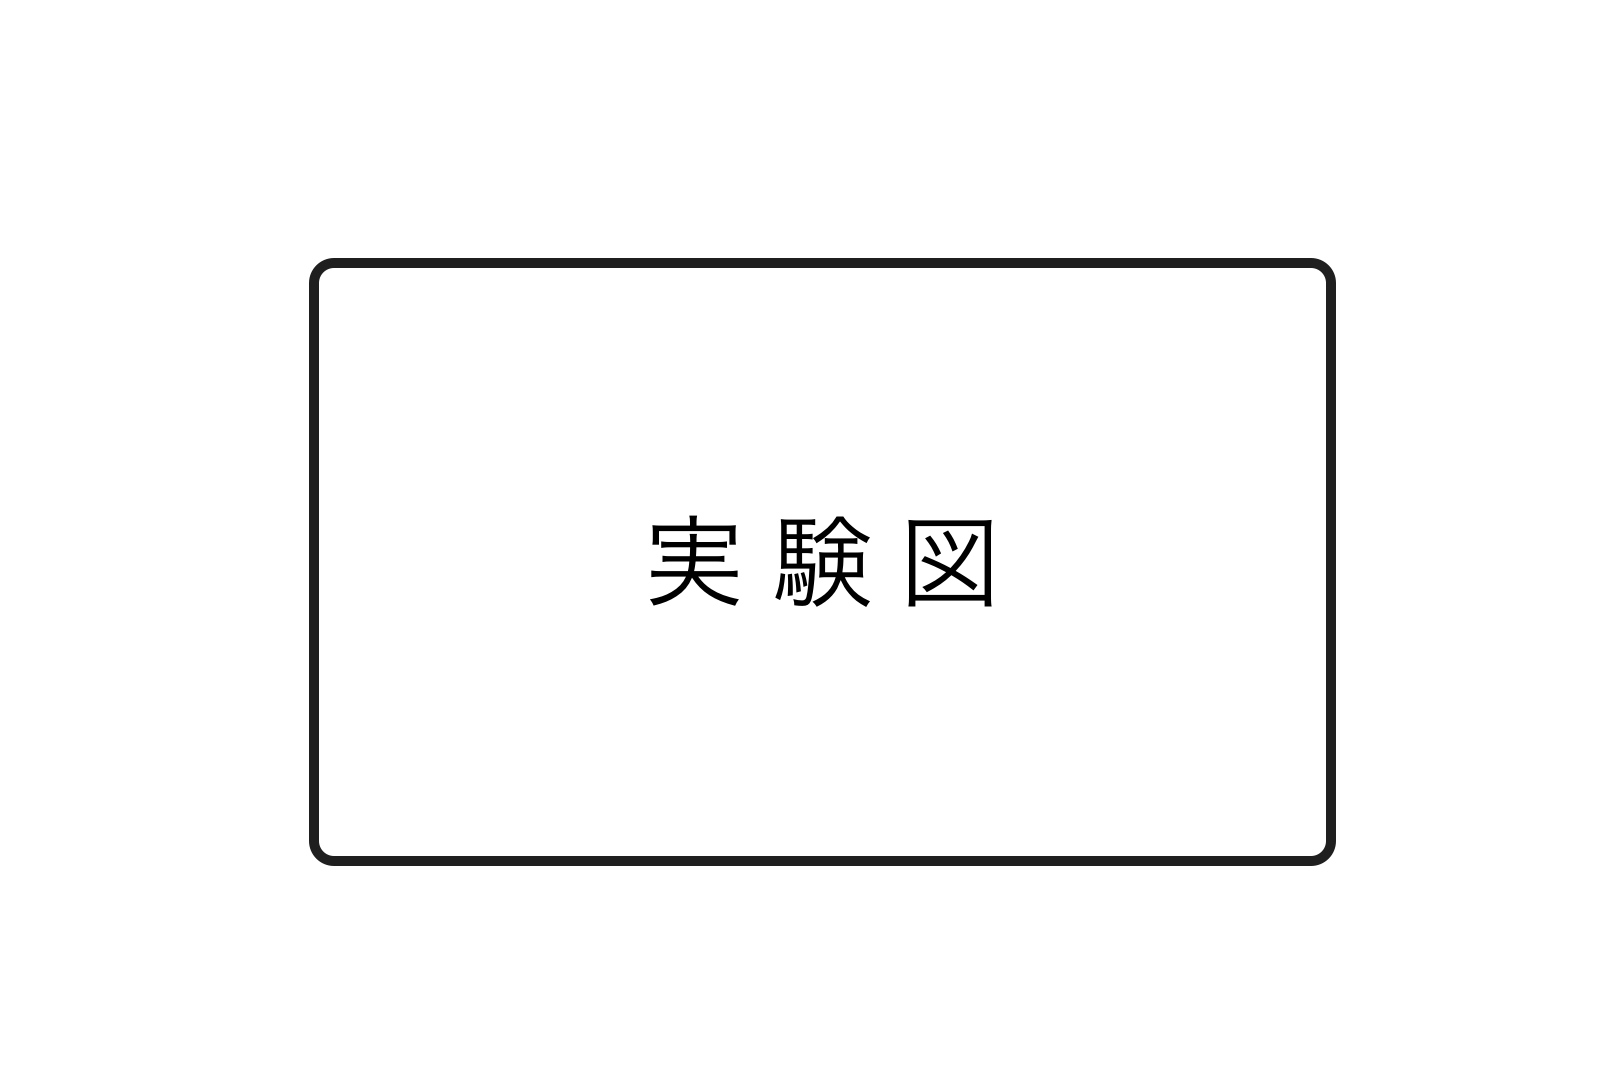
\includegraphics[width=7.5cm]{showcaseimage.png}
  \caption{実験の模式図}
  \label{fig:experiment-blender-nbg}
\end{figure}

\section{実験結果}
次のようなcsvファイルを考えることにします(これはランダムなデータで実際の実験とは関係がないです).
\lstinputlisting{src/data/e_showcase.csv}
\verb|src/data/make_table.py|を実行することにより,次の\reftab{tab:py_generals}を得ます.これはコマンドラインで\verb|make table.o|とすることでも生成できます.
\begin{table}[H]
\centering
\caption{Showcase(数式$T_\mathrm{A}$)}
\label{tab:py_generals}
\begin{tabular}{cc}
\toprule
  時間 $t$ / \si{s} &  水温$T$ / \si{\celsius} \\
\midrule
          0.000000 &                   16.0 \\
          7.265949 &                   19.0 \\
          7.427011 &                   22.0 \\
         10.888379 &                   22.0 \\
         10.956777 &                   23.0 \\
         13.025393 &                   25.0 \\
         14.409749 &                   26.0 \\
         19.995210 &                   26.0 \\
         22.724879 &                   27.0 \\
         23.235187 &                   29.0 \\
\bottomrule
\end{tabular}
\end{table}

生成された.texファイルは,\verb|\begin{table}[H]
\centering
\caption{Showcase(数式$T_\mathrm{A}$)}
\label{tab:py_generals}
\begin{tabular}{cc}
\toprule
  時間 $t$ / \si{s} &  水温$T$ / \si{\celsius} \\
\midrule
          0.000000 &                   16.0 \\
          7.265949 &                   19.0 \\
          7.427011 &                   22.0 \\
         10.888379 &                   22.0 \\
         10.956777 &                   23.0 \\
         13.025393 &                   25.0 \\
         14.409749 &                   26.0 \\
         19.995210 &                   26.0 \\
         22.724879 &                   27.0 \\
         23.235187 &                   29.0 \\
\bottomrule
\end{tabular}
\end{table}
|とすることで本文中に取り込めます.


同一のcsvファイルからgnuplotを用いてグラフを生成することもできます.グラフは\verb|make table.o|とするか,\verb|src/data|へと行き,gnuplotのファイルを実行することで得られます.
\begin{figure}[H]\centering
  \begin{tikzpicture}[gnuplot]
%% generated with GNUPLOT 5.4p2 (Lua 5.4; terminal rev. Jun 2020, script rev. 114)
%% Fri Feb 18 11:27:21 2022
\path (0.000,0.000) rectangle (12.500,8.750);
\gpcolor{color=gp lt color border}
\gpsetlinetype{gp lt border}
\gpsetdashtype{gp dt solid}
\gpsetlinewidth{1.00}
\draw[gp path] (2.813,0.985)--(2.993,0.985);
\draw[gp path] (10.270,0.985)--(10.090,0.985);
\node[gp node right] at (2.629,0.985) {$16$};
\draw[gp path] (2.813,2.050)--(2.993,2.050);
\draw[gp path] (10.270,2.050)--(10.090,2.050);
\node[gp node right] at (2.629,2.050) {$18$};
\draw[gp path] (2.813,3.115)--(2.993,3.115);
\draw[gp path] (10.270,3.115)--(10.090,3.115);
\node[gp node right] at (2.629,3.115) {$20$};
\draw[gp path] (2.813,4.180)--(2.993,4.180);
\draw[gp path] (10.270,4.180)--(10.090,4.180);
\node[gp node right] at (2.629,4.180) {$22$};
\draw[gp path] (2.813,5.246)--(2.993,5.246);
\draw[gp path] (10.270,5.246)--(10.090,5.246);
\node[gp node right] at (2.629,5.246) {$24$};
\draw[gp path] (2.813,6.311)--(2.993,6.311);
\draw[gp path] (10.270,6.311)--(10.090,6.311);
\node[gp node right] at (2.629,6.311) {$26$};
\draw[gp path] (2.813,7.376)--(2.993,7.376);
\draw[gp path] (10.270,7.376)--(10.090,7.376);
\node[gp node right] at (2.629,7.376) {$28$};
\draw[gp path] (2.813,8.441)--(2.993,8.441);
\draw[gp path] (10.270,8.441)--(10.090,8.441);
\node[gp node right] at (2.629,8.441) {$30$};
\draw[gp path] (2.813,0.985)--(2.813,1.165);
\draw[gp path] (2.813,8.441)--(2.813,8.261);
\node[gp node center] at (2.813,0.677) {$0$};
\draw[gp path] (4.304,0.985)--(4.304,1.165);
\draw[gp path] (4.304,8.441)--(4.304,8.261);
\node[gp node center] at (4.304,0.677) {$5$};
\draw[gp path] (5.796,0.985)--(5.796,1.165);
\draw[gp path] (5.796,8.441)--(5.796,8.261);
\node[gp node center] at (5.796,0.677) {$10$};
\draw[gp path] (7.287,0.985)--(7.287,1.165);
\draw[gp path] (7.287,8.441)--(7.287,8.261);
\node[gp node center] at (7.287,0.677) {$15$};
\draw[gp path] (8.779,0.985)--(8.779,1.165);
\draw[gp path] (8.779,8.441)--(8.779,8.261);
\node[gp node center] at (8.779,0.677) {$20$};
\draw[gp path] (10.270,0.985)--(10.270,1.165);
\draw[gp path] (10.270,8.441)--(10.270,8.261);
\node[gp node center] at (10.270,0.677) {$25$};
\draw[gp path] (2.813,8.441)--(2.813,0.985)--(10.270,0.985)--(10.270,8.441)--cycle;
\node[gp node center,rotate=-270] at (1.969,4.713) {水温$T$ / \si{\celsius}};
\node[gp node center] at (6.541,0.215) {時間$t$ / s	};
\gpcolor{rgb color={0.580,0.000,0.827}}
\gpsetpointsize{4.00}
\gp3point{gp mark 1}{}{(2.813,0.985)}
\gp3point{gp mark 1}{}{(4.980,2.583)}
\gp3point{gp mark 1}{}{(5.028,4.180)}
\gp3point{gp mark 1}{}{(6.061,4.180)}
\gp3point{gp mark 1}{}{(6.081,4.713)}
\gp3point{gp mark 1}{}{(6.698,5.778)}
\gp3point{gp mark 1}{}{(7.111,6.311)}
\gp3point{gp mark 1}{}{(8.777,6.311)}
\gp3point{gp mark 1}{}{(9.591,6.843)}
\gp3point{gp mark 1}{}{(9.744,7.908)}
\gpcolor{color=gp lt color border}
\node[gp node right] at (8.802,8.107) {$f(t)$};
\gpcolor{rgb color={0.000,0.620,0.451}}
\draw[gp path] (8.986,8.107)--(9.902,8.107);
\draw[gp path] (2.813,1.501)--(2.883,1.564)--(2.953,1.627)--(3.023,1.689)--(3.093,1.752)%
  --(3.163,1.815)--(3.233,1.878)--(3.303,1.941)--(3.373,2.004)--(3.443,2.066)--(3.513,2.129)%
  --(3.583,2.192)--(3.653,2.255)--(3.723,2.318)--(3.793,2.381)--(3.863,2.443)--(3.933,2.506)%
  --(4.003,2.569)--(4.073,2.632)--(4.143,2.695)--(4.213,2.758)--(4.283,2.820)--(4.353,2.883)%
  --(4.423,2.946)--(4.493,3.009)--(4.563,3.072)--(4.633,3.135)--(4.703,3.197)--(4.773,3.260)%
  --(4.843,3.323)--(4.913,3.386)--(4.983,3.449)--(5.053,3.512)--(5.123,3.574)--(5.193,3.637)%
  --(5.263,3.700)--(5.333,3.763)--(5.403,3.826)--(5.473,3.889)--(5.543,3.951)--(5.613,4.014)%
  --(5.683,4.077)--(5.753,4.140)--(5.823,4.203)--(5.893,4.266)--(5.963,4.328)--(6.033,4.391)%
  --(6.103,4.454)--(6.173,4.517)--(6.243,4.580)--(6.313,4.643)--(6.383,4.705)--(6.453,4.768)%
  --(6.523,4.831)--(6.593,4.894)--(6.663,4.957)--(6.733,5.020)--(6.803,5.082)--(6.873,5.145)%
  --(6.943,5.208)--(7.013,5.271)--(7.083,5.334)--(7.153,5.397)--(7.223,5.459)--(7.293,5.522)%
  --(7.363,5.585)--(7.433,5.648)--(7.503,5.711)--(7.573,5.774)--(7.643,5.836)--(7.713,5.899)%
  --(7.783,5.962)--(7.853,6.025)--(7.923,6.088)--(7.993,6.151)--(8.063,6.213)--(8.133,6.276)%
  --(8.203,6.339)--(8.273,6.402)--(8.343,6.465)--(8.413,6.528)--(8.483,6.590)--(8.553,6.653)%
  --(8.623,6.716)--(8.694,6.779)--(8.764,6.842)--(8.834,6.904)--(8.904,6.967)--(8.974,7.030)%
  --(9.044,7.093)--(9.114,7.156)--(9.184,7.219)--(9.254,7.281)--(9.324,7.344)--(9.394,7.407)%
  --(9.464,7.470)--(9.534,7.533)--(9.604,7.596)--(9.674,7.658)--(9.744,7.721);
\gpcolor{color=gp lt color border}
\draw[gp path] (2.813,8.441)--(2.813,0.985)--(10.270,0.985)--(10.270,8.441)--cycle;
%% coordinates of the plot area
\gpdefrectangularnode{gp plot 1}{\pgfpoint{2.813cm}{0.985cm}}{\pgfpoint{10.270cm}{8.441cm}}
\end{tikzpicture}
%% gnuplot variables

  \caption{Showcase of gnuplot}
  \label{fig:showcase}
\end{figure}
生成された.texファイルは,figure environmentで囲った上で\verb|\input|することで本文中に取り込めます.


\section{考察}
% Points
%  - 標準的な値との比較検討
%  - 気がついたこと,特に失敗したこと
%  - 実験に関して興味を持ったこと
%  - 原理式の導出

.bibファイルを使いたくなりますが,大学のフォーマットが独特なので大人しく\verb|thebibliography|を使った方が早いかもしれないです\footnote{bstファイルを作ることで独自のフォーマットを作成することができます.latex makebstでググってみてください.}.


\begin{thebibliography}{9}
\end{thebibliography}

\end{document}
